% Project 2 - EECS 499
% Author: Shaun Howard (smh150@case.edu)
\documentclass[conference]{IEEEtran} \usepackage[T1]{fontenc} \usepackage[backend=biber, style=ieee]{biblatex}
\addbibresource{report.bib} \usepackage[final]{microtype}

% graphics
\ifCLASSINFOpdf \usepackage[pdftex]{graphicx} % declare the path(s) where your graphic files are
  \graphicspath{{images/}} % and their extensions so you won't have to specify these with
  % every instance of \includegraphics
  \DeclareGraphicsExtensions{.jpeg,.png} \else
\fi

\usepackage{amsmath}
\usepackage[linesnumbered,ruled]{algorithm2e}
\usepackage{comment}
\usepackage[noend]{algpseudocode}

\newcommand{\sfunction}[1]{\textsf{\textsc{#1}}}
\algrenewcommand\algorithmicforall{\textbf{foreach}}
\algrenewcommand\algorithmicindent{.8em}

\begin{document}

\title{Multi-threaded Jacobian Pseudo-inverse RRT Path Planner with Randomized-IK Restarts for Baxter Dual Arm Manipulator}

\author{
 \IEEEauthorblockN{Shaun Howard}
 \IEEEauthorblockA{Electrical Engineering and Computer Science Department\\
                   Case Western Reserve University\\ 
                   Cleveland, Ohio 44106\\
                   Email: smh150@case.edu}
}

% make the title area
\maketitle

% As a general rule, do not put math, special symbols or citations
% in the abstract
\begin{abstract}
Within this paper, we present a flexible, multi-threaded solution to the motion planning problem for dual-armed robots with 7 degrees of freedom (DOF). The task of motion 
planning for robots with high DOF is computationally intensive due to the number of possible joint angle solutions in configuration and workspace along with avoiding nearby 
obstacles in motion plans. Building an RRT was time consuming for computer hardware of the past, but modern hardware allows for multiple processes to be run and communicate 
asynchronously with each other while executing computationally hard tasks. The algorithm presented in this paper is a sampling-based path planning algorithm that builds on the 
Jacobian Pseudo-inverse-Based Rapidly-exploring Random Tree (RRT) algorithm. The goal extension step for building the tree utilizes the popular Jacobian Pseudo-inverse (JPINV)
with various goal-based constraints on accepted solutions. However, unlike other planners, the random extension step in this planner utilizes random Inverse Kinematics 
restarts to plan for solutions based on random guesses to the IK solver for a given goal pose. This paper outlines the better properties of both JPINV and IK methods, while 
attempting to cut the costs of downsides for both planner methods by applying multi-threaded programming. The solution performs quickly and parallelizes the tasks that took
previous planners much more time. Our algorithm is compared to results of the JT, JPINV and random IK approaches to the RRT path planning technique.
\end{abstract}

\section{Introduction} \label{Introduction}

The search for accurate and quick planning algorithms has grown in recent years with major breakthroughs in memory architecture, processing unit speed and 
parallel processing. Several planning methods exist that intricately check environment surroundings, configuration space and workspace constraints, and validate
that solutions can be executed by the robot due to joint limits and constraints. These planners may or may not be able to cope with dynamic environment updates
without starting over entirely. The generation of solutions that are valid within a small window of time before the surrounding environment obstacles update
is a valuable trait of a modern motion planner.

Sampling-based algorithms were developed to randomly-generate solutions that meet the constraints of task being executed for some probability of motion planning time, while 
approaching the goal for the remaining period of time. A primary sampling-based approach to motion planning is the Rapidly-exploring Random Tree (RRT). Several motion planning
implementations utilize the RRT as proposed in \cite{rand_kin_planning}, \cite{anytime_rrts}, \cite{random_planner_wo_ik}, \cite{humanoid_motion_planning}, and many more. In the 
RRT algorithm, an initial joint configuration is provided as the start node. The planner grows randomly from the start node while sampling from the search space to grow the tree 
toward unexplored regions. Given that this planner can be biased to plan toward a goal configuration and handles high-dimensional search space well, it is suitable for motion
planning with high DOF kinematics chains. 

For the purposes of this paper, we wish to plan from a starting joint configuration to a  goal configuration, which can change over time, by generating a suitable and minimal
trajectory for the robot to execute the task at hand. Despite the simplicity of the original RRT algorithm, the constraints enforced on this problem along with performance needs
require modifications to be made to the original algorithm. Not only is there a workspace goal for the RRT to meet, but there are environmental obstacles and joint limit 
constraints imposed on the robot arm. Due to the large number of configuration space solutions to reach a particular Cartesian endpoint for a redundant manipulator, sampling plays 
a substantial role in reaching solutions quickly. These solutions may need tailoring to fit grasp orientation needs, which increases search time and complexity. Without
an exceptional amount of time, a good estimate of the optimal node at any particular time can often be provided to reach the workspace goal in configuration space with the RRT. 
Unfortunately, mapping workspace goals to configuration space goals does not have a simple solution of a closed-form for advanced high DOF manipulators, therefore RRT
modifications were developed to exploit the Jacobian as a mapping from configuration space to workspace as in \cite{random_planner_wo_ik}.

In this paper, an extension of the Jacobian Pseudoinverse-based RRT is made to include Inverse Kinematics in the random extension step of RRT construction.
The purpose of using IK to determine a valid random node configuration is to assure that random solutions are reachable. As a result, the algorithm can leverage the random 
nature of the RRT with a goal-directed extension that can quickly reach the goal by exploiting the Jacobian nature to link the configuration and workspace.
The works related to the planner described in this paper are outlined in the next section. Following, the problem for dual-arm motion planning is established. 
After that, sensor measurements and capturing data with the Kinect setup are discussed. Later, the implementation is discussed along with experimentation and 
simulator set up. Second to last, experimentation results are analysed and compared. Lastly, the paper is concluded with the results of the experiments.

\begin{figure}
\label{pic1} 
\centering 
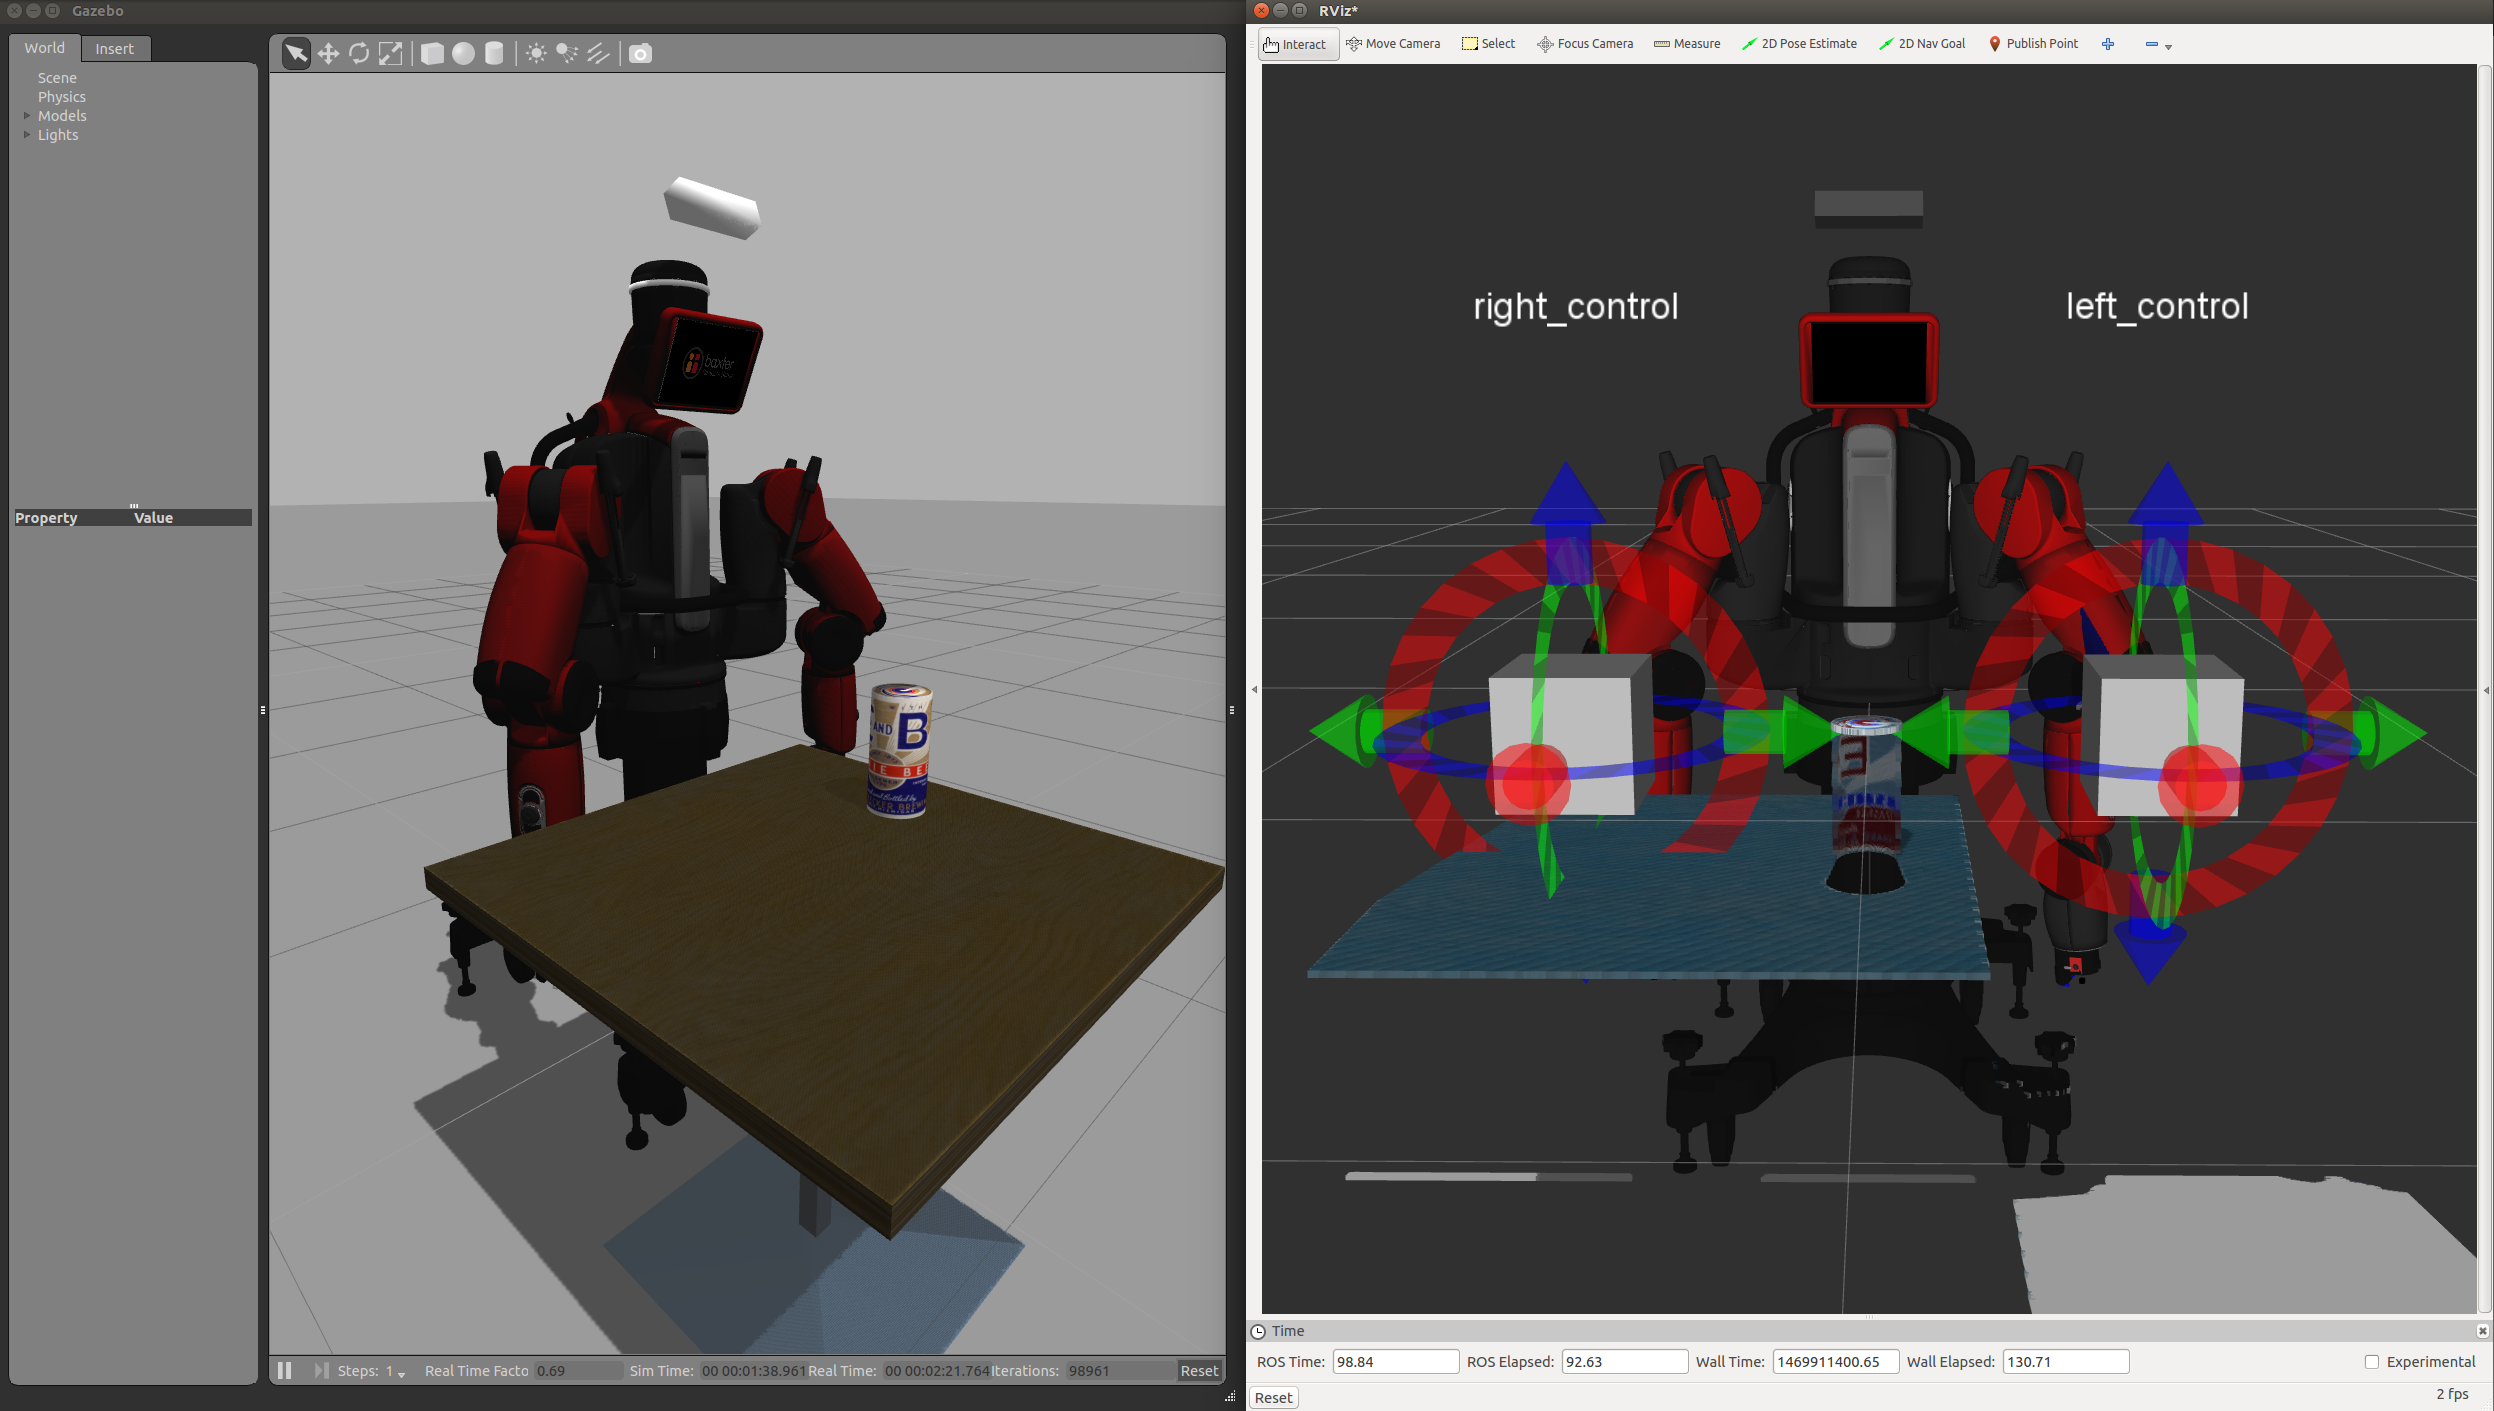
\includegraphics[width=0.49\textwidth]{sim1}
\caption{The Baxter simulator set-up with the Microsoft Xbox Kinect and some objects useful for obstacle detection in the scene.}
\end{figure}

\section{Related Work} \label{Related Work}

The RRT-JT planner was implemented in \cite{random_planner_wo_ik}. The paper combines the idea of an RRT with the usage of a goal-directed modification to 
the typical RRT algorithm, pulling the end effector to the goal with a certain probability, while randomly extending for the remainder of time. A valuable 
aspect of the planner described in the paper is that it does not rely on an IK solver. This method is quite useful when IK solvers would be infeasible to use
for high DOF robots. The planner implemented in the paper is highly based on that in \cite{integrated_path_planning} due to its nature of avoiding the use of
IK for random goal extensions. As mentioned in the paper, the planner in \cite{integrated_path_planning} selects "the configuration in the search tree that 
is closest to the workspace goal using a workspace distance metric and then extend out from this configuration in a random direction." Several advantages
of this method are mentioned, including avoiding inaccurate solutions due to inaccurate IK solvers and faster convergence to the goal than the standard RRT
algorithm. The method implemented in \cite{random_planner_wo_ik} goes even further by extending to the goal with a certain probability using jacobian
transpose. The paper mentions that although this method is useful, joint limits are an issue. Joint limits cause the use of the RRT-JT method to not be
independent, thus requiring some sort of alternative planner or restart method when solutions cannot be found.

In \cite{humanoid_motion_planning}, several novel methods for motion planning are presented. A novel IK solver is presented that utilizes gradient descent
in reachability spaces computed ahead of time and sampling of parameters in order to execute one or two arm query tasks. In terms of grasping objects,
end effector poses are sought to lead to appropriate grasps for the object at hand and also be collision free in the workspace. The planner they propose
is highly performance-oriented and requires a mere tens of milliseconds to solve a task query in contrast to iterative IK algorithms. One of the foreseeable downsides
to this method is that it uses pre-defined grasp poses to randomly extend in the workspace. Such pre-defined grasps would take quite a bit of effort to pre-compute
for each object in the workspace and translate to the configuration space.

The upcoming section describes the problem solved in this paper by using both the JPINV and random IK solver methods in one RRT.

\section{Problem Formulation} \label{Problem Formulation}

The problem at hand is the ability to solve motion planning tasks for high DOF robots with obstacle avoidance and little computational time. The JT addition to the typical RRT
construct provides a goal-directed approach to motion planning, rather than an exhaustive random search. This allows the planner to reach the goal in a shorter amount of time, 
making the RRT planning method more useful for real-time applications. The problem with the RRT-JT approach is that joint limits are met fairly quickly. The descent approach used 
in this process also takes quite an amount of time to converge to the solution since the JT steps are small. \cite{humanoid_motion_planning} discusses the weaknesses of the JT 
method, including those mentioned. Previous methods have shown that the JPINV and IK solvers each had their own upsides and downsides. The upsides of the JPINV is that it is easy 
to approximate a solution to the problem by using gradient descent, but as downsides, there are singularities and joint limits that can be encountered, effectively disabling the 
planner. The upsides of the IK planners is that they provide feasible solutions and perform search for you. The downsides of IK solvers are reaching singularities and not finding a 
possible solution configuration for a given workspace goal although more than one exist. These problems can be overcome by repetitively checking for IK solutions at random points 
within a limited distance step from the goal until a solution is found. 

The planner described in this paper is a versatile planner that has several options for planning. The first option is the JT paired with random IK extensions. The algorithm 
for the RRT-JT from \cite{random_planner_wo_ik} influenced the JT planner implemented in this paper. While this method's computational time is small and plans are accurate, it's 
planning capabilities are somewhat limited. The second option, the JPINV paired with random IK, adds more versatility to the planner. The JPINV planner utilized in this paper is 
influenced by multiple sources, primarily \cite{humanoid_motion_planning}. The JPINV may become stuck at joint limits, but such is rare and is typically overcome by the random 
nature of the IK planner to extend from the closest node in the RRT to unexplored space. This method is a bit slow in descending to the goal, so a speed-up is implemented
that uses the psuedo-inverse of the pseudo-inverse to make step sizes more concise to the goal.

Given the problems of detecting workspace obstacles, experimenting with algorithms, and testing algorithm execution, a test bed with simulator capabilities is needed. 
A test bed is built for testing these algorithms with the Gazebo simulator, Rviz, and the Microsoft Xbox Kinect for Point Cloud environment visualization. An 
obstacle avoidance collision checker is added to detect obstacles and plan in avoidance of them during RRT construction. The RRT construction pattern is to create the entire tree 
and prune nodes, then to execute the path. Although this type of planner usually assumes a static environment, the planner in this paper plans in accordance with real-time
obstacle updates from the Xbox Kinect. The planner framework presented in this paper updates obstacles at each available point in time in an asynchronous fashion from the planner. 
This decouples the obstacle detection from the planner, which greatly improves performance over existing planner designs. Obstacle detection and point cloud filtering functionality 
is provided with a ROS node intentionally created to update Kinect obstacle clouds for the robot, using various filters to publish a valid obstacle cloud for each robot arm.

The Baxter robot has two 7 degree of freedom (DOF) arms. A multi-threaded extension was added to the planner to allow for simultaneous construction of left and right arm
RRTs while still checking for obstacle collisions and workspace constraints when validating solutions. The obstacle collision checker filters 
each arm from its own obstacle cloud when possible. This allows each arm to plan in accordance for the other arm, to avoid collisions. The experiments 
with the planner described in this paper isolate each arm from the other for testing accuracy and speed on complex goal poses. Poses ranging from easy to 
complex are tested and compared. The Jacobian PINV method paired with random IK extensions turned out to be the most effective and efficient method for motion 
planning with both arms as it is implemented in a multi-threaded fashion, allowing the algorithm to harness the parallelized computational power of a modern computer
while still retaining the ability to solve for constraints imposed on the system by using the ROS publish/subscribe methodology.

Overall, the solutions to most of these problems include the application of multi-threading and asynchronous updates, separating methods that are computationally 
intensive or rely on time series data into their own nodes or threads in the planner program.

\section{Methodology} \label{Methodology}

The planner proposed solves some of the problems presented in the problem formulation section above. Most of the problems stem from hardware requirements, lack of parallel 
processing, and inability to combine multiple planning algorithms together due to performance constraints in older computing systems. The planner designed in this paper 
parallelizes the computationally intensive methods into their own nodes or processing threads in the program for the robot. It utilizes both the JPINV and random IK methods
of motion planning for nodes in a modified RRT construction algorithm based on those in \cite{random_planner_wo_ik} and \cite{humanoid_motion_planning} with the random extension
step modified to use a variant of the typical RRT random extension step with the IK RRT algorithm in mind. The determination of workspace obstacles is an important factor
in motion planning and will be further explored to come. The capture and filtering of environment point cloud data is covered in the next subsection.

\subsection{Sensor Measurements} \label{Sensor Measurements}

The Microsoft Xbox Kinect is used to collect point cloud data about the robot environment in the experiments. The point clouds are red-green-blue-depth (RGB-D) clouds. 
Thus, the color and depth information can be read and processed for filtering out points from the clouds to do pre-processing steps on them before they reach the robot. 
The points are received in the kinect\_pc\_frame, however almost all planning algorithms are based on goal poses in the robot base frame. Thus, the points must be 
transformed from the kinect\_pc\_frame to the base frame in order to make any sense to the robot's planners. Following, the immediate workspace cloud is constructed of 
points filtered above a certain z-position, since Baxter's arms cannot quite reach the floor on any usual base. The points can easily be filtered in x,y,z minimum and 
maximum ranges. The point of such filtering is to speed up image processing and obstacle detection time, thus in turn speeding up planning time as well. Each arm is 
considered its own unit of execution, thus it has its own thread. Each arm has different obstacle regions than the other because one arm is the obstacle
of another arm. Thus, it is useful for each arm to have its own filtered obstacle cloud. 

The left arm's obstacle cloud should have the left arm filtered out. The right arm's obstacle cloud should have the right arm filtered out of it. If these obstacle
clouds are updated frequently and the planner can update its obstacle regions for each arm to plan with on-demand, then this method of filtering is a part of the solution
to the problem of real-time planning in dynamic environments that the papers described thus far have lacked. The idea to do real-time updates stems from experimentation
with the RRT concept. Obstacle determination from point cloud data can be decoupled from the RRT construction algorithm, so the RRT only has to check if a configuration is in 
collision with the current obstacles, but it does not have to compute where the obstacles are beforehand. The thought of this de-coupling brings in the concept of a time series 
data model, where obstacle clouds are updated at each possible time step. The planner shall receive and update itself with the latest obstacles over time with planning. Thus, the 
planner solutions are based on random samples and are never the same again, but a solid improvement in the overall speed of the RRT planner with obstacle detection using both JPINV 
and IK algorithms is made by separating nodes in this way.

The idea of updating obstacles asynchronously, on-demand provides the ability to parallelize arm-planning and speed up the entire motion planning process tremendously.
This idea also allows data sharing between planner threads for most of the pre-processed workspace points, saving computational space, time and work. Not only did previous papers 
lack the ability of asynchronously updating obstacles, but they treated the environment statically during RRT construction. In modern applications, a static environment
assumption would crumble the foundation of the RRT solution, especially since RRTs can be slow for more complex trajectories and goal poses. The planner in this paper
has a hook to the asynchronous obstacle updates and receives the latest filtered obstacle clouds for the designated arm in order to provide the concept of dynamic 
obstacle avoidance to the extent of speed that the obstacle filtering node can unpack, update, transform and filter the environment point cloud for each arm, 
performing such operations on hundreds of thousands of four-dimensional RGB-D data points that designate the environment for the robot.
 
\subsection{Planner Design}

The planner design in this paper is inspired by the better qualities of the planners described in the papers mentioned in the related work section. Modifications were made to the 
concept of a Rapidly-exploring Random Tree in order for it to use both a random IK extension within a constrained Cartesian step size from the nearest configuration in the tree and 
a JPINV goal-directed extension with a certain probability, p\_goal, to decrease the convergence time of the algorithm. The hybrid RRT-JPINV algorithm with random IK extensions
will be discussed within the next subsections.

\subsection{RRT-JT and RRT-JPINV with Random IK Restarts}

The inspiration for random IK restarts with the RRT-JT planner came from the idea of stochastic processes. The RRT-JT planner can get stuck in local minima or reach joint
limits like most other Jacobian-based planners. A great addition to undermine the predetermined nature of getting stuck in minima for the planner would be to add random
restarts somehow. One of the more convenient and reliable ways of doing so would be to add random IK restarts. These random IK restarts would not be sampled from a database,
but points would be randomly generated in a range increasing over time with execution. The benefit of doing so would be that the planner would always be able to climb out of local
minima during gradient descent due to the randomness of the RRT random extend step which is uniformly-selected with a probability of 1-p\_goal, where p\_goal is the probability 
of the planner extending to the goal with either the JT or JPINV algorithms. As infants experiment with things until they get the answer they
want about why something happens as in cause and effect, the planner would randomly guess when randomly extending to a node with the random-point IK solver would be a good idea.
An addition to this would be to have a set of heuristics to determine when to switch planners for planner turnaround minimization. However, currently, a the probability
p\_goal is the deciding factor to switch between the random extension step and the goal extension step of the planner. The JPINV method is also a part of the planner which
can be toggled to replace the JT. All the Jacobian-related options are condensed into one algorithm with boolean flags in the planner.

The following is pseudo-code for the extend\_toward\_goal method which uses either the JT or JPINV for goal-directed planning.

\begin{algorithm}
    \SetKwInOut{Input}{Input}
    \SetKwInOut{Output}{Output}

    \underline{function Euclid} $(dist\_thresh, time\_limit)$\;
    \Input{$dist\_thresh$ in meters, $time\_limit$ in seconds}

     \State $\mathit{q\_old} \gets closest\_node\_to\_goal$
     \State $first\gets\true$
     \begin{comment}
     Q\_new = []
     prev\_dist\_to\_goal = self.dist\_to\_goal()
     current\_milli\_time = get\_curr\_time\_in\_ms()
     curr\_time = current\_milli\_time()
     prev\_time = curr\_time
     \While {prev\_dist\_to\_goal > dist\_thresh and curr\_time - prev\_time < time\_limit}
         x\_old = self.fwd\_kin(q\_old)
         dx = self.workspace\_delta(x\_old)
         if use\_adv\_gradient\_descent:
             J = self.kin.jacobian(q\_old)
             if use\_pinv:
                 JT = np.linalg.pinv(J)
             else:
                 JT = J.T
             direction = np.dot(JT, np.dot(J, JT)**-1)
         else:
             if use\_pinv:
                 JT = self.kin.jacobian\_pinv(q\_old)
             else:
                 JT = self.kin.jacobian\_transpose(q\_old)
             direction = JT
         dq = np.dot(direction, dx)
         q\_new = q\_old + dq
         curr\_dist\_to\_goal = self.\_dist\_to\_goal(self.fwd\_kin(q\_new))
         if curr\_dist\_to\_goal < prev\_dist\_to\_goal and math.fabs(curr\_dist\_to\_goal-prev\_dist\_to\_goal) < max\_dist\_cap\
                 and self.collision\_checker.collision\_free(q\_new):
             self.exec\_angles(q\_new)
             Q\_new.append(q\_new)
             q\_old = q\_new
             prev\_dist\_to\_goal = curr\_dist\_to\_goal
         else:
             break
	\end{comment}
    \caption{Euclid's algorithm for finding the greatest common divisor of two nonnegative integers}
\end{algorithm}

       

The random IK restart step pseudo-code for the method ik\_extend\_randomly is as follows:
\begin{comment}
        Q_new = []
        prev_dist_to_goal = self.dist_to_goal()
        num_tries_left = num_tries
        first = True
        # start with soln at offset and work away from goal
        curr_diameter = offset
        while prev_dist_to_goal > dist_thresh and num_tries_left > 0:
            goal_pose = self.get_goal_pose()
            if first:
                first = False
                # first, try the goal point
                next_point = self.goal_point()
            else:
                goal_arr = self.goal_node()
                next_point = []
                for i in range(3):
                    curr_coord = curr_pos[i]
                    goal_coord = goal_arr[i]
                    radius = curr_diameter/2.0
                    if curr_coord < goal_coord:
                        next_point.append(h.generate_random_decimal(curr_coord-radius, goal_coord+radius))
                    else:
                        next_point.append(h.generate_random_decimal(goal_coord-radius, curr_coord+radius))
            print "looking for ik soln..."
            if self.collision_checker.check_collision(next_point, avoidance_radius):
                next_pose = h.generate_goal_pose_w_same_orientation(next_point, goal_pose.orientation)
                solved, q_new = ik_soln_exists(next_pose, self.kin)
                if solved:
                    curr_dist_to_goal = self._dist_to_goal(self.fwd_kin(q_new))
                    curr_pos = next_point
                    # only add the point as a soln if the distance from this point to goal is less than that from the
                    # last end effector point
                    if curr_dist_to_goal < prev_dist_to_goal and self.collision_checker.collision_free(q_new):
                        print "random ik planner: curr dist to goal: " + str(curr_dist_to_goal)
                        self.exec_angles(q_new)
                        Q_new.append(q_new)
                        prev_dist_to_goal = curr_dist_to_goal
                        continue
                    else:
                        print "ik: soln not collision free..."
                else:
                    print "could not find ik soln for generated point"
            # increment current range for generating random points by adding another offset amount
            curr_diameter += offset
            num_tries_left -= 1
        self.add_nodes(Q_new)
\end{comment}
\subsection{RRT-JPINV with Random IK Restarts}


inspiration: realtime rrt, learning by doing


\subsection{Planner Implementation} \label{Planner Implementation}

\subsection{Gazebo Simulation} \label{Gazebo Simulation}
 A Gazebo simulation paired with Rviz is used to examine custom implementations of the algorithms mentioned. 
 
\section{Results} \label{Results}
A comparison is made between the methods used 
during experimentation which reveals that the hybrid RRT planner is quicker than the other planning methods while balancing constraints and generating a viable solution to 
almost any problem within reach of the given end effector in use.

\section{Conclusion} \label{Conclusion} 
This method was found to perform better than the Jacobian-Transpose and IK-based approaches overall, although 
each method has upsides and downsides. Rarely, if ever, does the planner get noticeably stuck in local minima unless a goal is impossible for the end effector to 
reach.

\subsection{Future Work}

\printbibliography
\end{document}